\documentclass[12pt,executivepaper]{article}
\usepackage[utf8]{inputenc}
\usepackage[spanish]{babel}
\usepackage{amsmath}
\usepackage{amsfonts}
\usepackage{amssymb}
\usepackage{graphics}
\usepackage{graphicx}
\usepackage[left=1cm,right=1cm,top=2cm,bottom=2cm]{geometry}
\usepackage{imakeidx}
\makeindex[columns=3, title=Alphabetical Index, intoc]
\usepackage{listings}
\usepackage{xcolor}
\usepackage{multicol}
\usepackage{changepage}
\usepackage{float}
\usepackage{cite}
\usepackage{url}
\usepackage{hyperref}
\usepackage{pdfpages}

\definecolor{codegreen}{rgb}{0,0.6,0}
\definecolor{codegray}{rgb}{0.5,0.5,0.5}
\definecolor{codepurple}{rgb}{0.58,0,0.82}
\definecolor{backcolour}{rgb}{0.95,0.95,0.92}

\lstdefinestyle{mystyle}{
    backgroundcolor=\color{backcolour},
    commentstyle=\color{codegreen},
    keywordstyle=\color{magenta},
    numberstyle=\tiny\color{codegray},
    stringstyle=\color{codepurple},
    basicstyle=\ttfamily\footnotesize,
    breakatwhitespace=false,
    breaklines=true,
    captionpos=b,
    keepspaces=true,
    numbers=left,
    numbersep=5pt,
    showspaces=false,
    showstringspaces=false,
    showtabs=false,
    tabsize=3
}

\lstset{style=mystyle}
\author{González Pardo Adrian}
\date{Marzo 2020}

\title{Reporte de practica 4}
\newcommand\tab[1][1cm]{\hspace*{#1}}
\begin{document}
\maketitle
\section{Código VHDL}
\begin{center}
    \lstinputlisting[language=VHDL]{./sources/sumador.vhd}
    \textit{Código fuente de sumador de 1 bit}\\
    \lstinputlisting[language=VHDL]{./sources/alu1.vhd}
    \textit{Código fuente de ALU de 1 bit}\\
    \lstinputlisting[language=VHDL]{./sources/AluN.vhd}
    \textit{Código fuente de la ALU de $m$ bits generalizada}
    
\end{center}
\section{Test-Bench VHDL Código}
\begin{center}
    \lstinputlisting[language=VHDL]{./sources/simAlumN.vhd}
    \textit{Código de simulación}\\
    \textbf{Anexo de fotos de la simulación a impulsos}
\end{center}
\begin{center}
    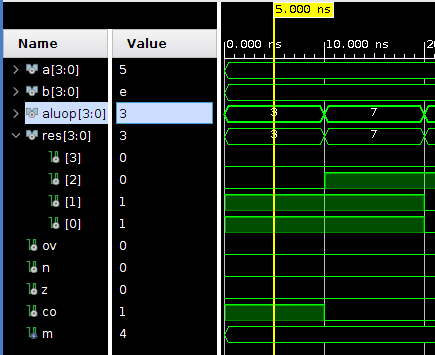
\includegraphics[scale=0.666]{imgs/uno.png}\\
    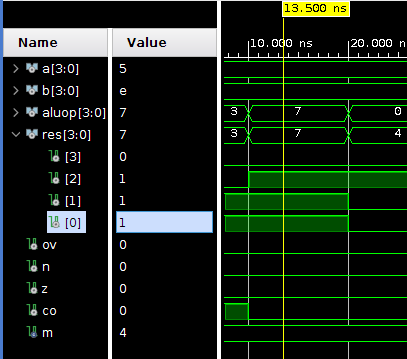
\includegraphics[scale=0.666]{imgs/dos.png}\\
    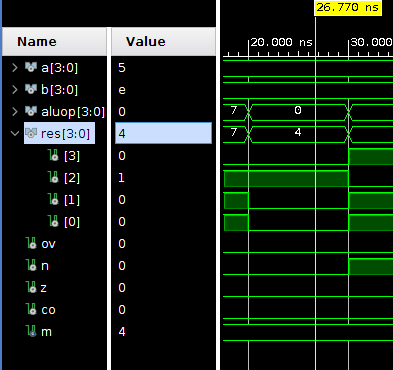
\includegraphics[scale=0.666]{imgs/tres.png}\\
    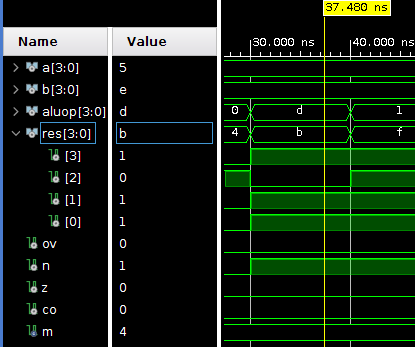
\includegraphics[scale=0.666]{imgs/cuatro.png}\\
    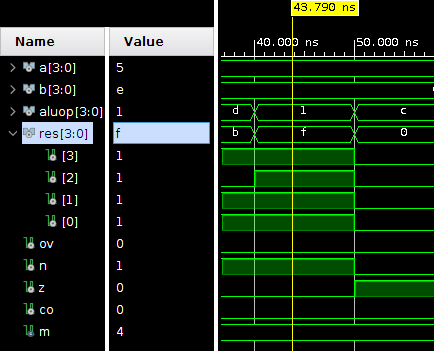
\includegraphics[scale=0.666]{imgs/cinco.png}\\
    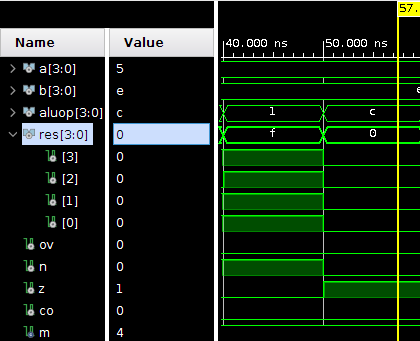
\includegraphics[scale=0.666]{imgs/seis.png}\\
    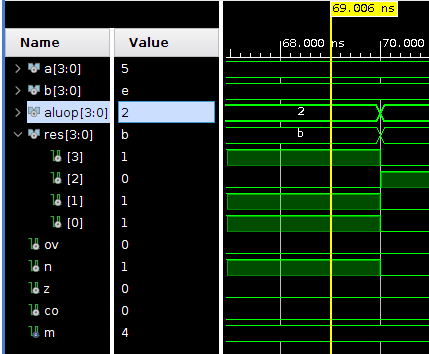
\includegraphics[scale=0.666]{imgs/siete.png}\\
    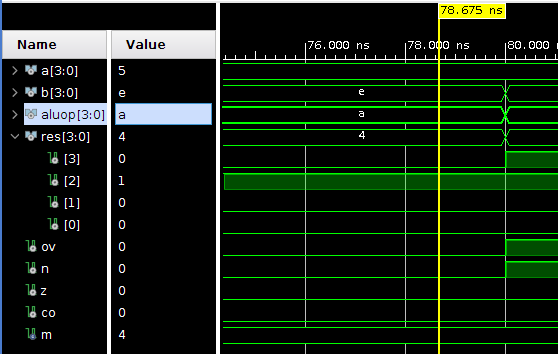
\includegraphics[scale=0.666]{imgs/ocho.png}\\
    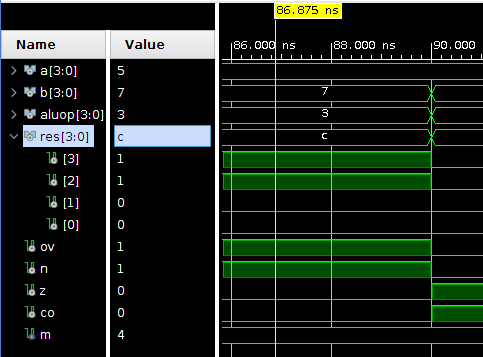
\includegraphics[scale=0.666]{imgs/nueve.png}\\
    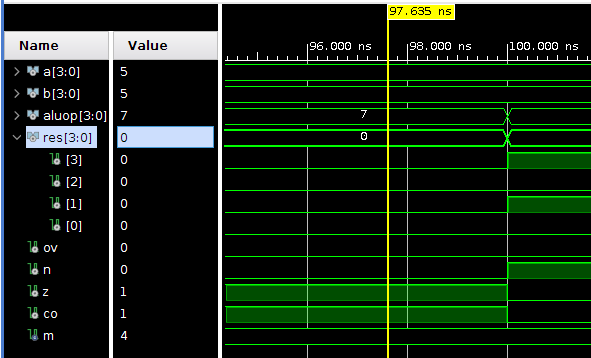
\includegraphics[scale=0.666]{imgs/diez.png}\\
    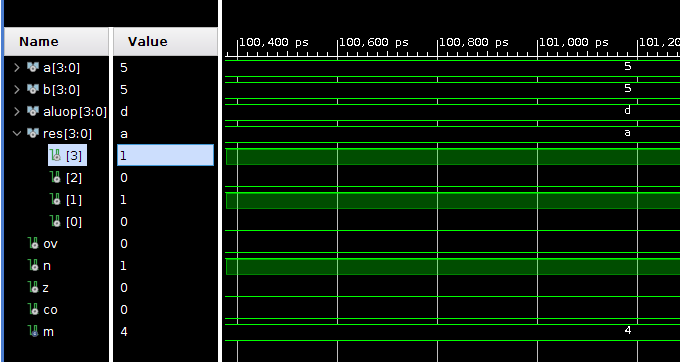
\includegraphics[scale=0.666]{imgs/once.png}
\end{center}

\section{Tabla de resultados}
\begin{center}
    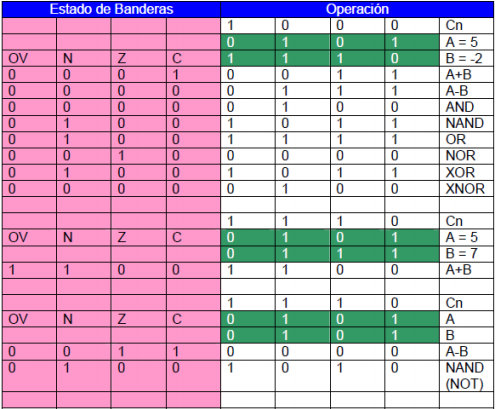
\includegraphics[scale=0.666]{imgs/tabla.png}\\
    \textbf{Figura: Tabla que concuerda con los resultados obtenidos en la simulación}
\end{center}
\clearpage
\section{Diagrama RTL}
\begin{center}
    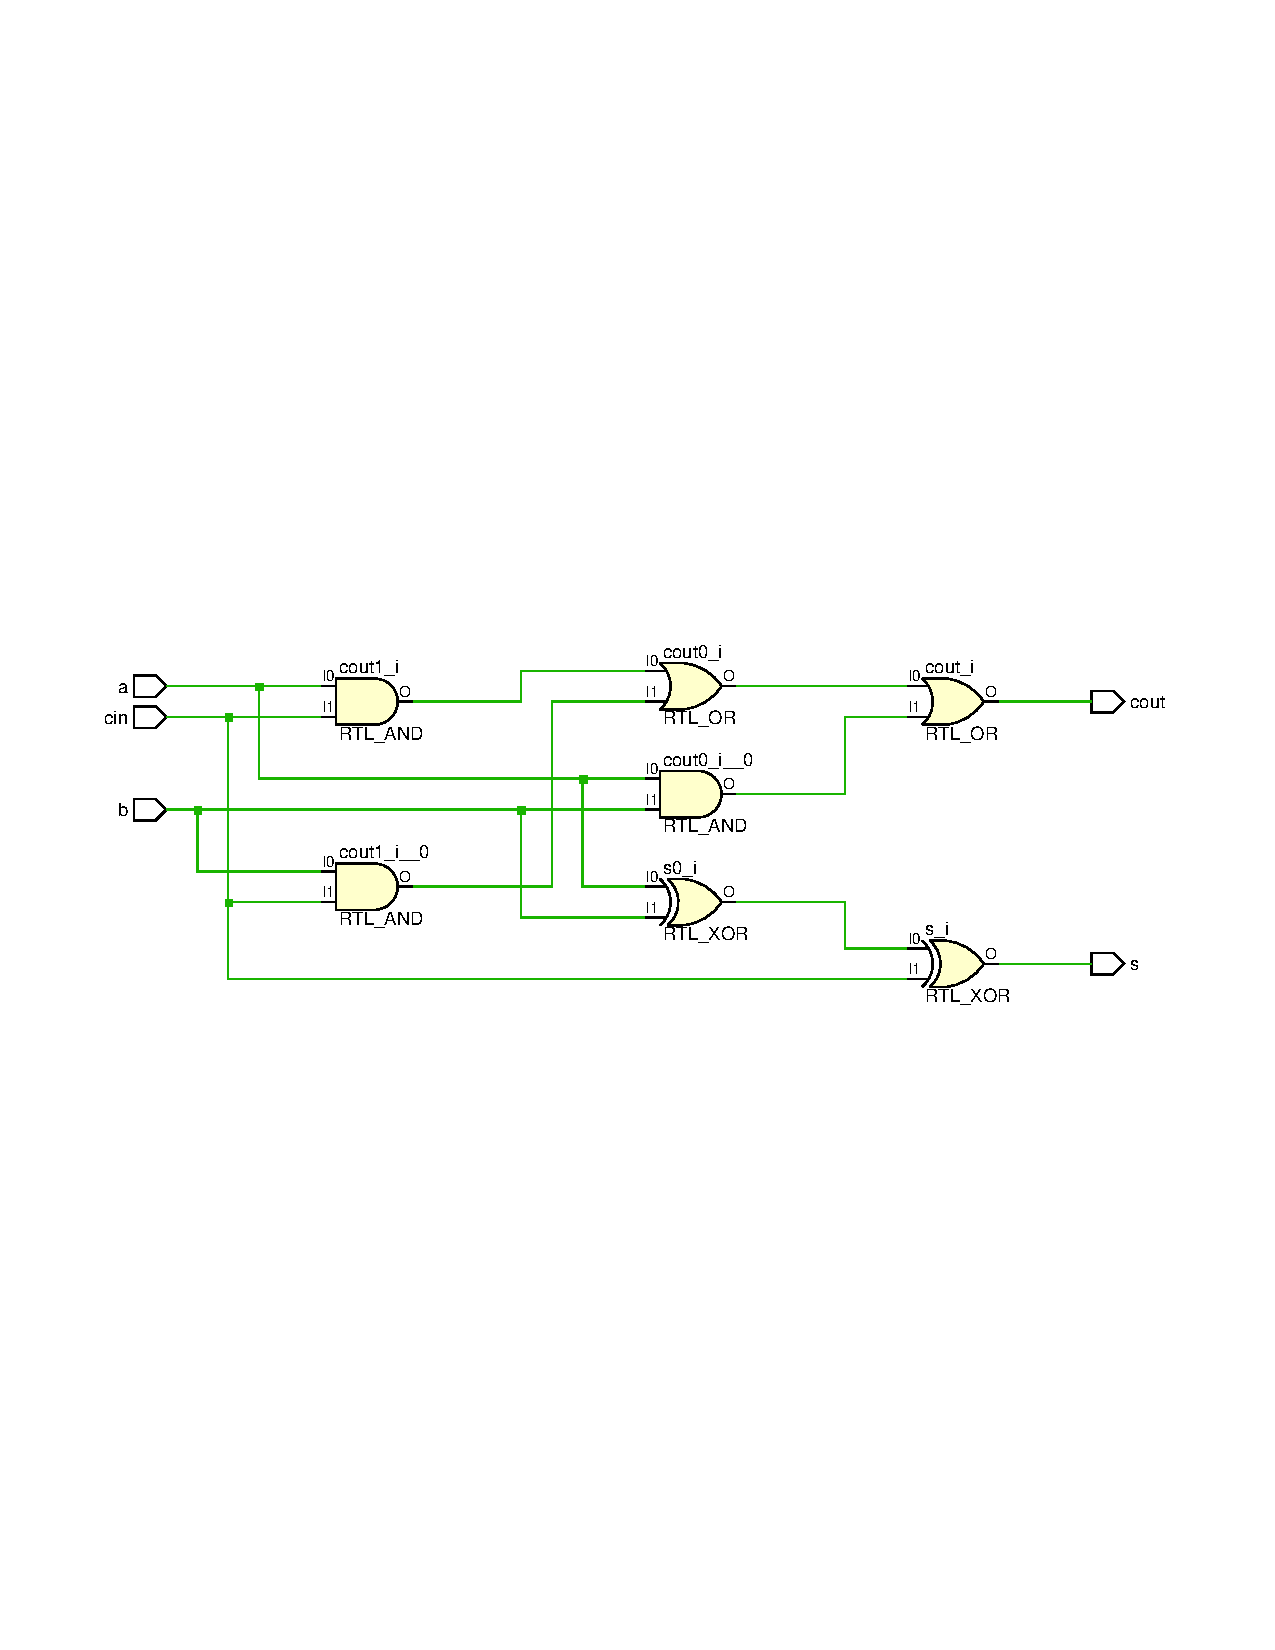
\includegraphics[scale=0.7]{sources/schematic-Sumador.pdf}
    \textit{Diagrama RTL del archivo VHDL del sumador de 1 bit}
    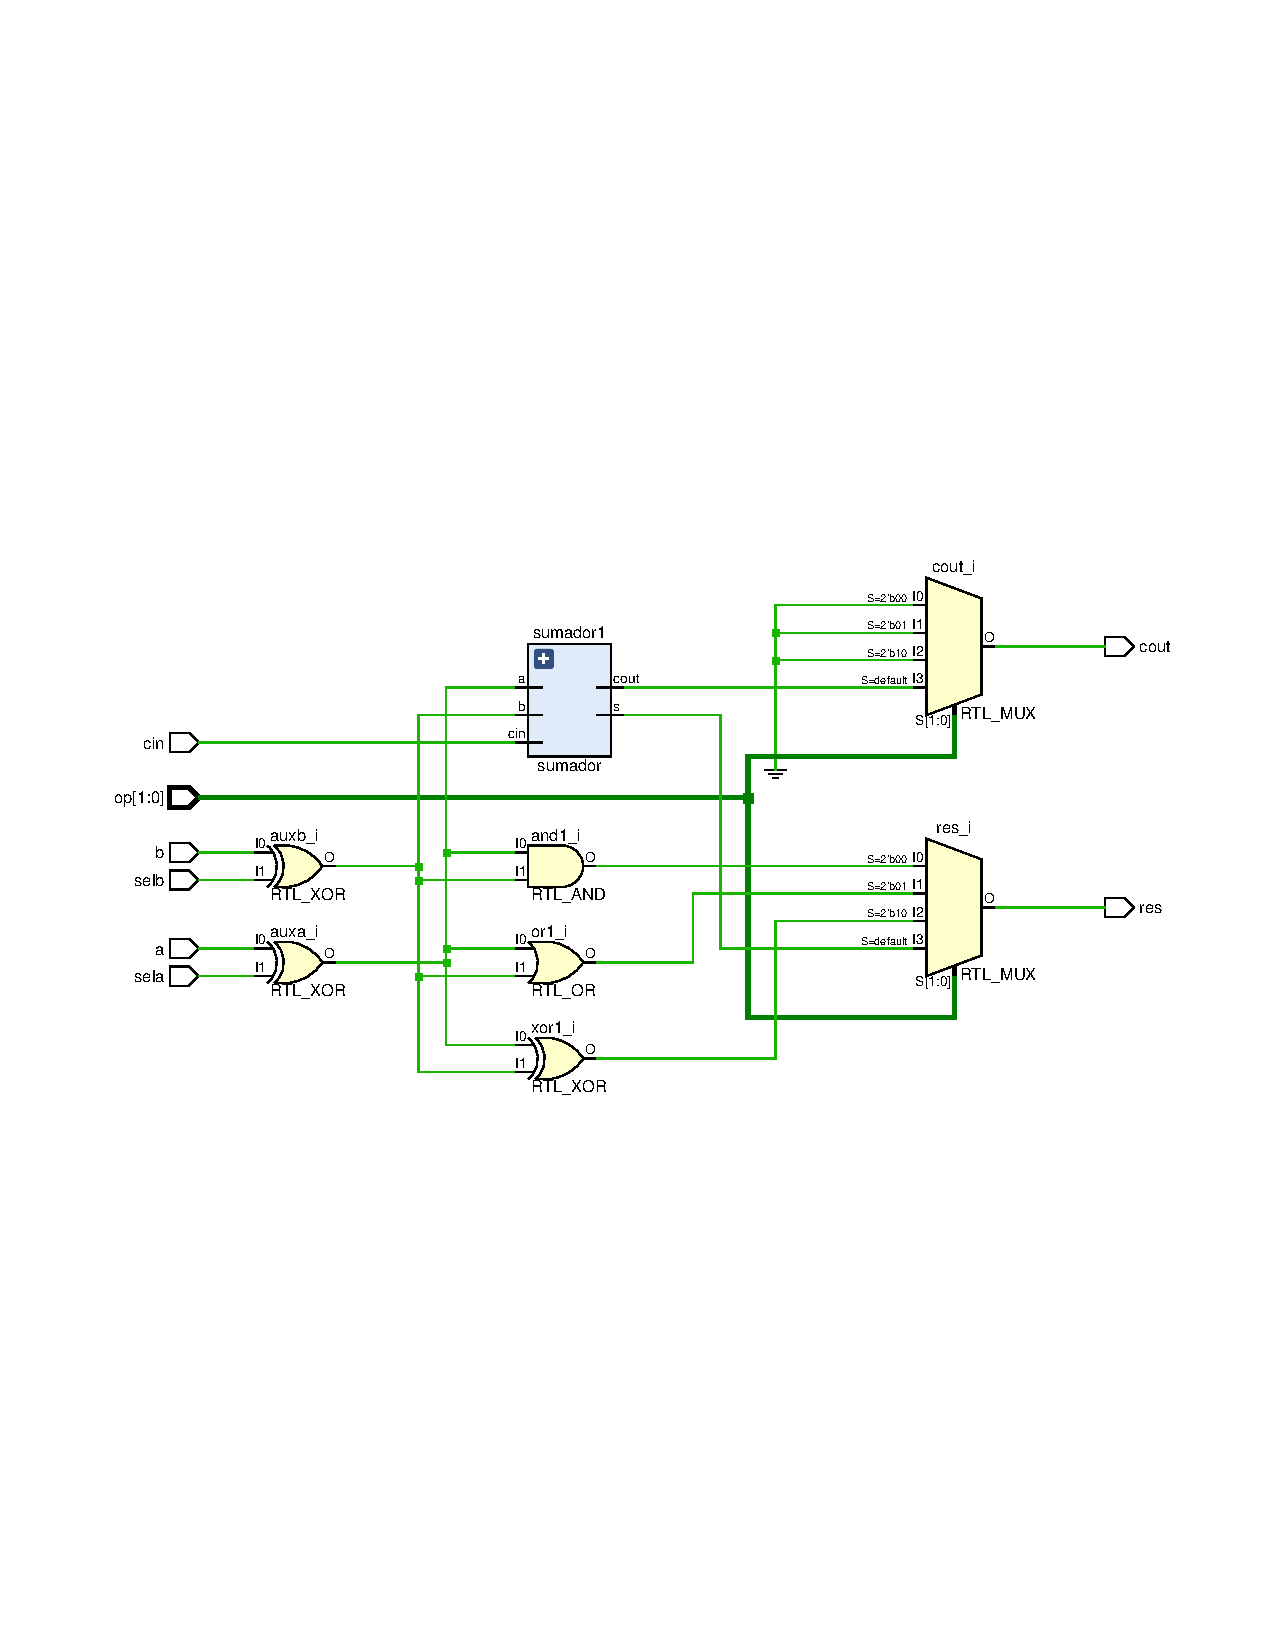
\includegraphics[scale=0.7]{sources/schematicRLT-ALU1.pdf}
    \textit{Diagrama RTL del archivo VHDL de la ALU de 1 bit}
    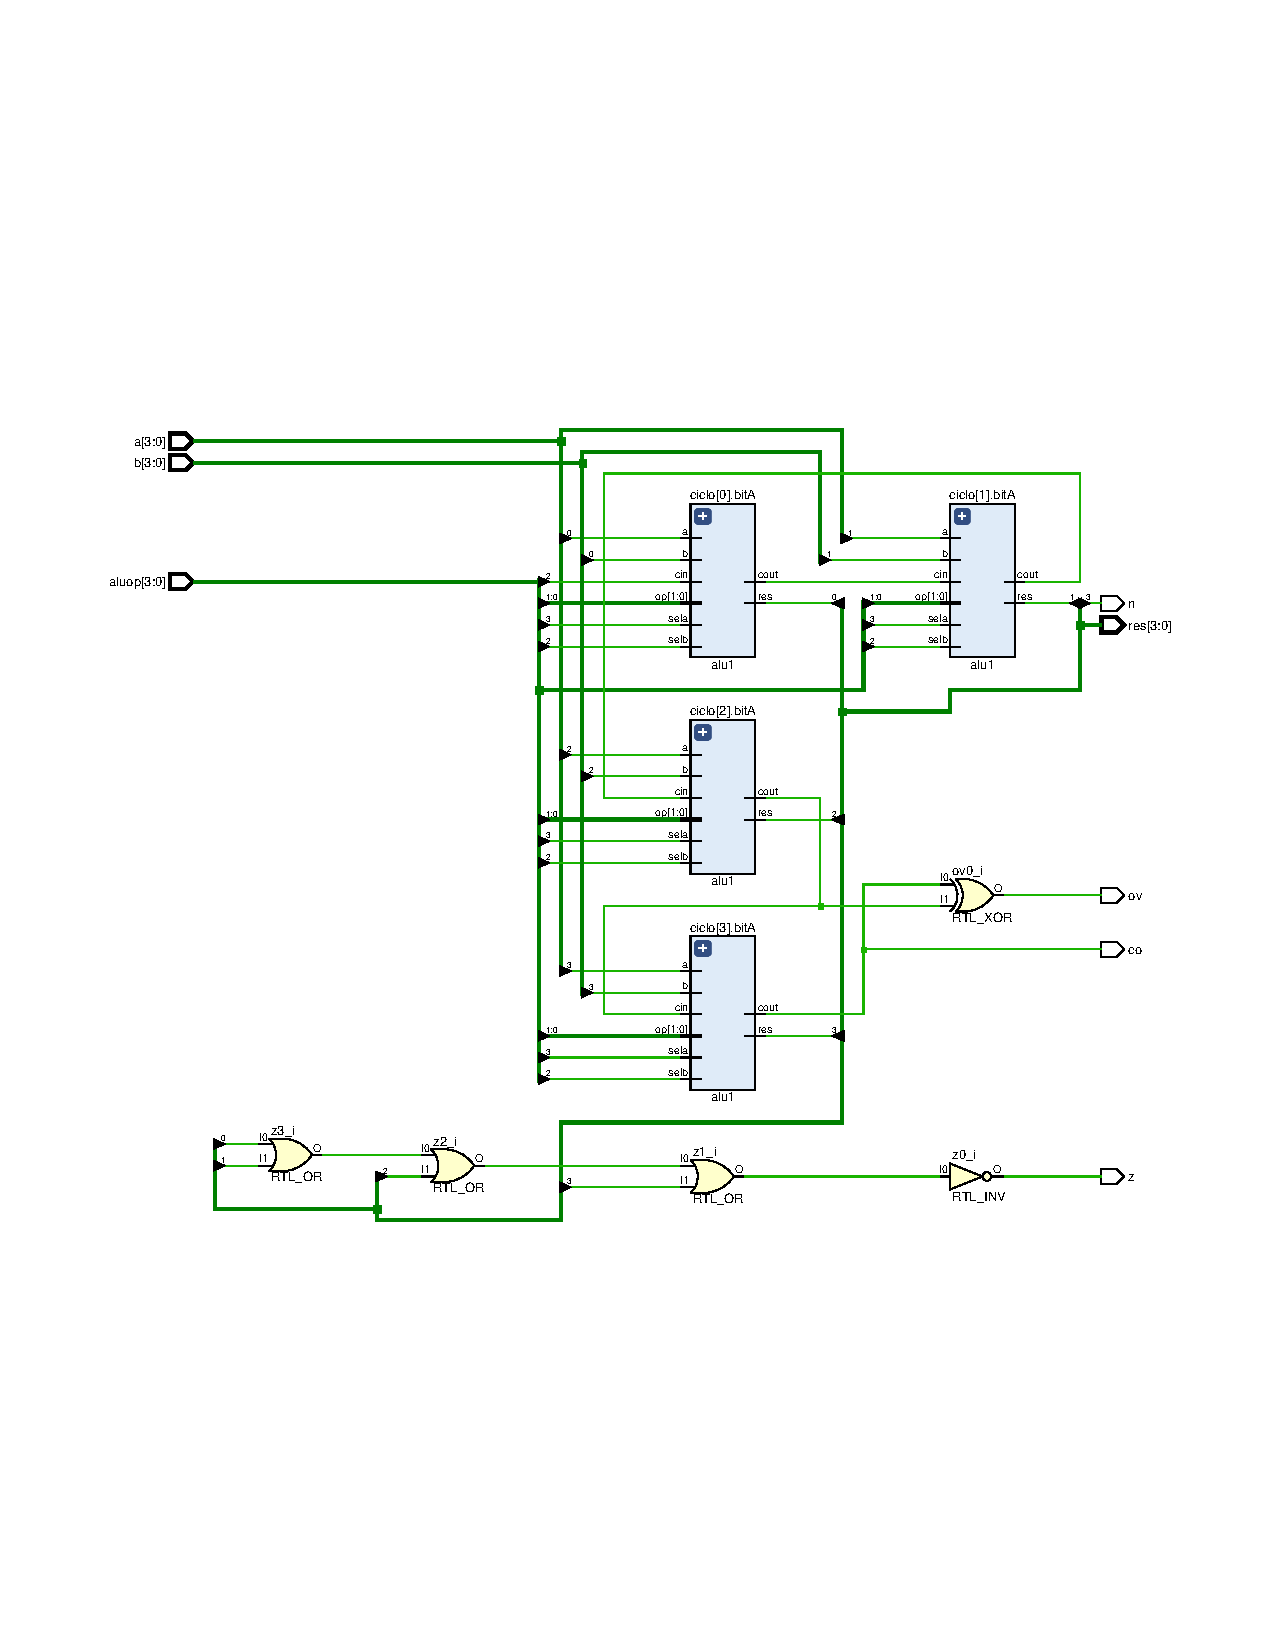
\includegraphics[scale=0.7]{sources/schematicRTL-ALUN.pdf}
    \textit{Diagrama RTL del archivo VHDL de la ALU de m bits}
\end{center}
\end{document}
